% comment out for student version
\ifdefined\Student\relax\else\def\Teacher{}\fi

\documentclass[12pt]{article}

\title{Activity 9: Software Development}
\author{Dr. Chris Mayfield}
\date{CS 101, Fall 2020}

%\ProvidesPackage{cspogil}

% fonts
\usepackage[utf8]{inputenc}
\usepackage[T1]{fontenc}
\usepackage{mathpazo}

% spacing
\usepackage[margin=2cm]{geometry}
\renewcommand{\arraystretch}{1.4}
\setlength{\parindent}{0pt}

% orphans and widows
\clubpenalty=10000
\widowpenalty=10000
\pagestyle{empty}

% figures and tables
\usepackage{graphicx}
\usepackage{multicol}
\usepackage{tabularx}
\usepackage{wrapfig}

% fixed-width columns
\usepackage{array}
\newcolumntype{L}[1]{>{\raggedright\let\newline\\\arraybackslash\hspace{0pt}}m{#1}}
\newcolumntype{C}[1]{>{\centering\let\newline\\\arraybackslash\hspace{0pt}}m{#1}}
\newcolumntype{R}[1]{>{\raggedleft\let\newline\\\arraybackslash\hspace{0pt}}m{#1}}

% include paths
\makeatletter
\def\input@path{{Models/}{../../Models/}}
\graphicspath{{Models/}{../../Models/}}
\makeatother

% colors
\usepackage[svgnames,table]{xcolor}
\definecolor{bgcolor}{HTML}{FAFAFA}
\definecolor{comment}{HTML}{007C00}
\definecolor{keyword}{HTML}{0000FF}
\definecolor{strings}{HTML}{B20000}

% table headers
\newcommand{\tr}{\bf\cellcolor{Yellow!10}}

% syntax highlighting
\usepackage{textcomp}
\usepackage{listings}
\lstset{
    basicstyle=\ttfamily\color{black},
    backgroundcolor=\color{bgcolor},
    numberstyle=\scriptsize\color{comment},
    commentstyle=\color{comment},
    keywordstyle=\color{keyword},
    stringstyle=\color{strings},
    columns=fullflexible,
    keepspaces=true,
    showlines=true,
    showstringspaces=false,
    upquote=true
}

% code environments
\newcommand{\java}[1]{\lstinline[language=java]{#1}}%[
\lstnewenvironment{javalst}{\lstset{language=java,backgroundcolor=}}{}
\lstnewenvironment{javabox}{\lstset{language=java,frame=single,numbers=left}\quote}{\endquote}

% PDF properties
\usepackage[pdftex]{hyperref}
\urlstyle{same}
\makeatletter
\hypersetup{
  pdftitle={\@title},
  pdfauthor={\@author},
  pdfsubject={\@date},
  pdfkeywords={},
  bookmarksopen=false,
  colorlinks=true,
  citecolor=black,
  filecolor=black,
  linkcolor=black,
  urlcolor=blue
}
\makeatother

% titles
\makeatletter
\renewcommand{\maketitle}{\begin{center}\LARGE\@title\end{center}}
\makeatother

% boxes [optional height]
\newcommand{\emptybox}[1][10em]{
\vspace{1em}
\begin{tabularx}{\linewidth}{|X|}
\hline\\[#1]\hline
\end{tabularx}}

% models
\newcommand{\model}[1]{\section{#1}\nopagebreak}
\renewcommand{\thesection}{Model~\arabic{section}}

% questions
\newcommand{\quest}[1]{\subsection*{Questions~ (#1)}}
\newcounter{question}
\newcommand{\Q}{\vspace{1em}\refstepcounter{question}\arabic{question}.~ }
\renewcommand{\thequestion}{\#\arabic{question}}

% sub-question lists
\usepackage{enumitem}
\setenumerate[1]{label=\alph*)}
\setlist{itemsep=1em,after=\vspace{1ex}}

% inline answers
\definecolor{answers}{HTML}{C0C0C0}
\newcommand{\ans}[1]{%
\ifdefined\Student
    \leavevmode\phantom{~~\textcolor{answers}{#1}}
\else
    ~~\textcolor{answers}{#1}
\fi}

% longer answers [optional height]
\newsavebox{\ansbox}
\newenvironment{answer}[1][4em]{
\nopagebreak
\begin{lrbox}{\ansbox}
\begin{minipage}[t][#1]{\linewidth}
\color{answers}
}{
\end{minipage}
\end{lrbox}
\ifdefined\Student
    \phantom{\usebox{\ansbox}}%
\else
    \usebox{\ansbox}%
\fi}


\begin{document}

\maketitle

Software development activities are grouped into four main categories: \emph{analyze}, \emph{design}, \emph{code}, and \emph{test}.
This activity explores ways to organize these categories into a software development life cycle (SDLC).

% based on Model A of Software Development Life Cycles by Clif Kussmaul

\model{Finding \& Fixing Errors}

Estimate how long (seconds, minutes, hours, days, weeks, months, or years) it typically takes to correct an error in software when it is found by:

\begin{center}
\begin{tabularx}{\textwidth}{|l|X|l|}
\hline
a. & a \textbf{compiler}, seconds after the file was edited
   & seconds
\\ \hline
b. & a \textbf{compiler}, later the same day or during a nightly build
   & hours/days
\\ \hline
c. & a \textbf{pair programming} partner, seconds after the error was made
   & \ans{seconds}
\\ \hline
d. & a \textbf{code review}, days or weeks after the file was edited
   & \ans{days/weeks}
\\ \hline
e. & a \textbf{customer} or other user, months after the software is released
   & \ans{months}
\\ \hline
f. & a \textbf{unit test}, minutes after the file was edited
   & \ans{minutes}
\\ \hline
g. & a \textbf{unit test}, later the same day or during a nightly build
   & \ans{hours/days}
\\ \hline
h. & a \textbf{system test}, shortly before software is released
     (weeks or months after the file was edited)
   & \ans{weeks/months}
\\ \hline
\end{tabularx}
\end{center}


\quest{5 min}


\Q Describe (or sketch a graph of) the relationship between the time to \textbf{find an error} and the time and cost to \textbf{repair an error}.

\begin{answer}[10em]
The longer it takes to find an error, the longer and more costly is is to repair.

NOTE: Ambler (2009) and Boehm (1978) contain graphs of this relationship.
\end{answer}


\Q Explain why we should use an SDLC that finds and fixes errors as quickly as possible.

\begin{answer}
The faster we find errors, the faster and less expensive it is to fix them.
\end{answer}

% based on Model B of Software Development Life Cycles by Clif Kussmaul

\model{The Waterfall Model}

The following diagram shows the typical percentage of \textbf{total cost \& effort} for each stage of software development.
In practice, these percentages vary widely by project.

\begin{center}
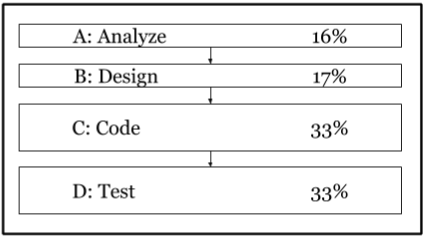
\includegraphics[scale=0.75]{waterfall.png}
\end{center}


\quest{10 min}


\Q Based on the Waterfall Model:

\begin{enumerate}%[itemsep=1ex]

\item How many stages are there?
\ans{4}

\item Which stage is 1st?
\ans{A:~Analyze}

\item Which stage(s) must be finished before \textbf{coding} starts?
\ans{A:~Analyze, B:~Design}

\end{enumerate}


\Q Based on the Waterfall Model:

\begin{enumerate}%[itemsep=1ex]

\item What \% of total effort is in the \textbf{last stage}?
\ans{33\%}

\item What \% of total effort is in the \textbf{first two stages}?
\ans{33\%}

\item When the project is \underline{25\%} completed, what \% of \textbf{analysis} is done?
\ans{100\%}

\item When the project is \underline{25\%} completed, what \% of \textbf{coding} is done?
\ans{0\%}

\item When the project is \underline{50\%} completed, what \% of \textbf{coding} is done?
\ans{About 50\%}

\item When the project is \underline{50\%} completed, what \% of \textbf{testing} is done?
\ans{0\%}

\end{enumerate}


\newpage

\Q It is important to find and fix errors in software.

\begin{enumerate}%[itemsep=1ex]

\item If \textbf{coding} errors are found during \textbf{C:~Code}, \\ in which stage should they be fixed?
\ans{C:~Code}

\item If \textbf{coding} errors are found during \textbf{D:~Test}, \\ in which stage should they be fixed?
\ans{D:~Test}

\item If \textbf{analysis} errors are found during \textbf{B:~Design}, \\ in which stage should they be fixed?
\ans{B:~Design}

\item If \textbf{analysis} errors are found during \textbf{D:~Test}, \\ in which stage should they be fixed?
\ans{D:~Test}

\item Which stage focuses most on \textbf{finding} errors?
\ans{D:~Test}

\item Are major errors in analysis and design more likely \\ when the project is \textbf{similar} to past projects, or \textbf{different}?
\ans{different}

\end{enumerate}


\Q Later stages often take more time, effort, and money than expected.
Explain why based on your answers to the previous questions.

\begin{answer}[5em]
Later stages must fix errors from earlier stages, and many errors are found late in the project during the Test stage.
\end{answer}

% based on Model C of Software Development Life Cycles by Clif Kussmaul

\model{The Iterative Model}

\begin{center}
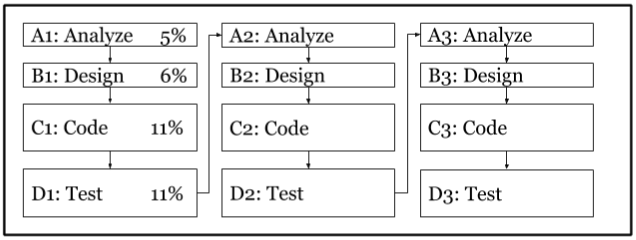
\includegraphics[scale=0.75]{iterative.png}
\end{center}

Assume that the total cost \& effort is the same for \ref{waterfall.tex} and \ref{iterative.tex}.
They differ only in how the SDLC is organized.


\quest{15 min}


\Q Based on the Iterative Model:

\begin{enumerate}%[itemsep=1ex]

\setlength{\defaultwidth}{15em}

\item How many stages are there?
\ans{12}

\item Which stage is 7th?
\ans{C2:~Code}

\item Which stages involve design?
\ans{B1, B2, B3}

\item What \% of total effort is for the \textbf{first four stages}?
\ans{33\% ~ A1+B1+C1+D1}

\item What \% of total effort is for \textbf{testing}?
\ans{33\% ~ D1+D2+D3}

\item What \% of total effort is for \textbf{analysis and design}?
\ans{33\% ~ A1+A2+A3 + B1+B2+B3}

\end{enumerate}


\Q Based on the Iterative Model:

\begin{enumerate}%[itemsep=1ex]

\setlength{\defaultwidth}{11em}

\item During what stage is the project \underline{25\%} completed?
\ans{D1}

\item When the project is \underline{25\%} completed, what \% of \textbf{analysis} is done?
\ans{33\% ~ A1 only}

\item When the project is \underline{25\%} completed, what \% of \textbf{coding} is done?
\ans{33\% ~ C1 only}

\item When the project is \underline{25\%} completed, what \% of \textbf{testing} is done?
\ans{About 9\% ~ (3\%/33\%)}

\item During what stage is the project \underline{50\%} completed?
\ans{C2}

\item When the project is \underline{50\%} completed, what \% of \textbf{analysis} is done?
\ans{67\% ~ A1 and A2}

\item When the project is \underline{50\%} completed, what \% of \textbf{coding} is done?
\ans{About 52\% ~ (17\%/33\%)}

\item When the project is \underline{50\%} completed, what \% of \textbf{testing} is done?
\ans{About 33\% ~ (11\%/33\%)}

\end{enumerate}


\vspace{1ex}
\comment{NOTE: The iterative model does not necessarily repeat exactly three times.
The key idea is that it repeats each stage multiple times, for the reasons you will identify on the next page.}

\newpage


\Q It is important to find and fix errors in software.

\begin{enumerate}%[itemsep=1ex]

\setlength{\defaultwidth}{8em}

\item If \textbf{analysis} errors are found during \textbf{A1:~Analyze}, \\ in which stage could they be fixed?
\ans{A1:~Analyze}

\item If \textbf{analysis} errors are found during \textbf{B1:~Design}, \\ in which stage could they be fixed?
\ans{A2:~Analyze}

\item If \textbf{coding} errors are found during \textbf{D2:~Test}, \\ in which stage could they be fixed?
\ans{C3:~Code}

\item If \textbf{analysis} errors are found during \textbf{B2:~Design}, \\ in which stage could they be fixed?
\ans{A3:~Analyze}

\item Are \textbf{analysis} errors likely to cause \textbf{design} errors?
\ans{Yes}

\item Are \textbf{design} errors likely to cause \textbf{coding} errors?
\ans{Yes}

\item Is it better to have \textbf{one try} or \textbf{several tries} \\ to remove all errors from the project?
\ans{several tries}

\end{enumerate}


\Q Explain why each test stage should try to find as many errors as possible.

\begin{answer}[5em]
The sooner you find a defect, (1) the easier it is to fix, and (2) the few other defects it causes.
\end{answer}


\Q Explain why \textbf{Iterative} is less likely then \textbf{Waterfall} to run into projects later in the project.

\begin{answer}[5em]
Iterative finds and fixes problems sooner, rather than waiting until the end of the life cycle.
\end{answer}


\end{document}
